%%%%%%%%%%%%%%%%%%%%%%%%%%%%%%%%%%%%%%%%%%%%%%%%%%%%%%%%%%%%%%%%%%%%%%%%%%%%%%%%
%% BAN TIENG VIET de gui co duyet (KHONG phai ban nop).
%% Template: Springer Nature sn-jnl. Can sn-jnl.cls trong cung thu muc / project.
%%
%% >>> QUAN TRONG: Bien dich bang pdfLaTeX (mac dinh Overleaf la duoc).
%%     Tieng Viet co dau hoat dong nho goi [vietnamese]{babel} + [T5]{fontenc}.
%%     Neu dau tieng Viet bi loi, doi compiler sang XeLaTeX trong:
%%     Overleaf -> Menu -> Settings -> Compiler -> XeLaTeX,
%%     roi thay 2 dong fontenc/babel ben duoi bang:
%%       \usepackage{fontspec}
%%       \usepackage{polyglossia}\setmainlanguage{vietnamese}
%%%%%%%%%%%%%%%%%%%%%%%%%%%%%%%%%%%%%%%%%%%%%%%%%%%%%%%%%%%%%%%%%%%%%%%%%%%%%%%%

\documentclass[pdflatex,sn-mathphys-num]{sn-jnl}

\usepackage{lmodern}
\usepackage[utf8]{inputenc}
\usepackage[T5]{fontenc}
\usepackage[vietnamese]{babel}

% Nhãn cấu trúc để tiếng Anh (babel mặc định dịch sang tiếng Việt); nội dung vẫn tiếng Việt
\addto\captionsvietnamese{%
  \renewcommand{\abstractname}{Abstract}%
  \renewcommand{\tablename}{Table}%
  \renewcommand{\figurename}{Fig.}%
  \renewcommand{\refname}{References}%
  \renewcommand{\bibname}{References}%
  \renewcommand{\appendixname}{Appendix}%
}

\usepackage{graphicx}
% Tìm hình trong thư mục figures/ HOẶC cùng cấp main_vi.tex (linh hoạt cho Overleaf)
\graphicspath{{figures/}{./}{../figures/}}
\usepackage{multirow}
\usepackage{amsmath,amssymb,amsfonts}
\usepackage{booktabs}

\usepackage{algorithm}
\usepackage{algpseudocode}

\usepackage{tabularx}
\usepackage{makecell}
\usepackage{array}
\newcolumntype{Y}{>{\centering\arraybackslash}X}
\newcolumntype{L}{>{\raggedright\arraybackslash}X}

\raggedbottom

\begin{document}

\title[Adaptive PB-JCI]{Adaptive Poisson-Binomial Joint Conformal Intervals for Reliable Cell Counting under Distribution Shift}

% \author*[1]{\fnm{Việt Hằng} \sur{Dương}}\email{hangdv@uit.edu.vn}

% \author[1]{\fnm{Thị Thu Hiệp} \sur{Đinh}}\email{250101085@grad.uit.edu.vn}

% \affil*[1]{\orgdiv{Faculty of Computer Science},
% \orgname{University of Information Technology (UIT), VNU-HCM},
% \orgaddress{\city{Ho Chi Minh City}, \country{Vietnam}}}
\author*[1]{\fnm{Anonymous} \sur{Author(s)}}
\affil*[1]{\orgdiv{Anonymous Department},
\orgname{Anonymous Institution},
\orgaddress{\city{Anonymous City}, \country{Anonymous Country}}}

\abstract{%
Đếm nhân tế bào trên ảnh mô bệnh học là bước quan trọng để xây dựng các chỉ dấu định
lượng trong computational pathology. Tuy nhiên, số đếm suy ra từ các mô hình phân vùng và
phát hiện hiện nay thường chỉ là một ước lượng điểm và chưa định lượng độ bất định, một
hạn chế đáng lo ngại khi dữ liệu triển khai bị dịch chuyển phân phối so với dữ liệu hiệu chỉnh.
Conformal prediction cho phép xây dựng khoảng dự đoán với bảo đảm coverage dưới giả
định trao đổi được, nhưng hiệu chỉnh tĩnh thường suy giảm dưới dịch chuyển, trong khi bài toán đếm đa lớp đòi hỏi phủ
đồng thời toàn bộ vector số đếm.

Chúng tôi đề xuất Adaptive PB-JCI Online, một tầng hiệu chỉnh conformal trực tuyến nhẹ
cho các backbone đếm tế bào sẵn có. Phương pháp mô hình hóa đóng góp của từng thực thể
bằng phân phối Poisson-Binomial để ước lượng thang phương sai giải tích, sử dụng thống
kê cực đại trên các lớp để hiệu chỉnh phủ đồng thời, và cập nhật ngưỡng bằng cửa sổ
trượt có kích thước thích nghi theo coverage quan sát gần đây. Trên ba bộ dữ liệu
PanNuke, NuInsSeg, MoNuSAC và hai backbone SAM3, PathoSAM, thành phần phủ đồng thời dựa
trên thống kê cực đại đạt \(91.7\%\) joint coverage trên MoNuSAC với \(K=4\) lớp. Dưới dịch chuyển có kiểm soát trên
PanNuke, phương pháp duy trì coverage gần mục tiêu trên SAM3 và cải thiện đáng kể
coverage trên PathoSAM, với khoảng dự đoán hẹp hơn ACI.
Trong dịch chuyển chéo bộ dữ liệu PanNuke \(\to\) NuInsSeg, nơi hiệu chỉnh tĩnh chỉ còn
khoảng \(41\%\) empirical coverage, cơ chế thích nghi khôi phục empirical coverage về
\(90.0 \pm 0.6\%\) và đạt điểm Winkler thấp nhất so với các baseline conformal trực
tuyến gần đây. Kết quả cho thấy tầng conformal đề xuất có thể bổ sung khoảng dự đoán
đáng tin cậy cho các hệ đếm tế bào dưới dịch chuyển phân phối.
}


\keywords{conformal prediction, uncertainty quantification, cell counting,
distribution shift, Poisson-Binomial, histopathology}
\maketitle

%==============================================================================
\section{Introduction}\label{sec:intro}

Đếm và phân loại nhân tế bào trên ảnh mô bệnh học nhuộm Hematoxylin và Eosin
(H\&E) là một bài toán nền tảng trong giải phẫu bệnh số. Nhiều chỉ dấu định lượng
quan trọng, chẳng hạn như mật độ tế bào hoặc tỉ lệ giữa các loại nhân, được suy ra
trực tiếp từ số lượng và thành phần tế bào trong mô. Gần đây, các mô hình nền tảng
cho phân vùng ảnh, tiêu biểu như Segment Anything~\cite{kirillov2023segment} và các
biến thể chuyên biệt cho mô bệnh học~\cite{archit2025patho}, đã giúp giảm đáng kể
chi phí chú giải bằng cách tạo ra các mặt nạ thực thể với rất ít dữ liệu gán nhãn
chuyên biệt. Từ các mặt nạ này, số lượng tế bào có thể được suy ra bằng cách tổng
hợp các thực thể đã phát hiện.

Tuy nhiên, các hệ thống đếm dựa trên phân vùng thường chỉ cung cấp một ước lượng
điểm cho số lượng tế bào mà không kèm theo định lượng độ bất định. Điều này là một
hạn chế quan trọng trong các ứng dụng y sinh, nơi người dùng không chỉ cần biết mô
hình dự đoán bao nhiêu tế bào, mà còn cần biết dự đoán đó đáng tin cậy đến mức nào.
Vấn đề trở nên nghiêm trọng hơn khi dữ liệu triển khai khác với dữ liệu hiệu chỉnh
do khác biệt về phòng xét nghiệm, quy trình nhuộm, thiết bị quét, hoặc loại mô. Trong
các trường hợp này, một mô hình có sai số trung bình chấp nhận được vẫn có thể tạo ra
các dự đoán quá tự tin trên những ảnh lệch miền.

Conformal prediction~\cite{vovk2005algorithmic, angelopoulos2023gentle} cung cấp một
khung thống kê để xây dựng khoảng dự đoán với bảo đảm coverage hữu hạn mẫu dưới giả
định trao đổi được giữa dữ liệu hiệu chỉnh và dữ liệu kiểm thử. Tuy nhiên, việc áp
dụng trực tiếp conformal prediction cho đếm tế bào đa lớp còn gặp hai khó khăn. Thứ
nhất, các bộ hiệu chỉnh tĩnh dựa trên một tập hiệu chỉnh cố định có thể suy giảm
coverage khi phân phối dữ liệu triển khai bị dịch chuyển~\cite{barber2023conformal,
gibbs2021adaptive}. Thứ hai, trong bài toán đa lớp, mục tiêu không chỉ là phủ đúng
từng lớp riêng lẻ, mà là phủ đồng thời toàn bộ vector số đếm. Hiệu chỉnh độc lập từng
lớp, chẳng hạn bằng hiệu chỉnh Bonferroni~\cite{dunn1961multiple}, có thể quá bảo thủ
hoặc không trực tiếp tối ưu cho sự kiện phủ đồng thời.

Trong nghiên cứu này, chúng tôi đề xuất Adaptive PB-JCI Online, một khung conformal
trực tuyến cho bài toán đếm tế bào đa lớp dưới dịch chuyển phân phối. Phương pháp
đầu tiên mô hình hóa đóng góp của từng thực thể vào số đếm lớp bằng xác suất
Poisson-Binomial, trong đó điểm objectness của thực thể được kết hợp với xác suất
lớp từ type head. Từ mô hình này, chúng tôi suy ra phương sai giải tích theo từng lớp
và sử dụng nó làm thang chuẩn hóa cho điểm bất hợp lệ. Tiếp theo, một thống kê cực
đại trên các lớp được dùng để xây dựng khoảng dự đoán phủ đồng thời. Cuối cùng, trong
thiết lập trực tuyến có phản hồi nhãn, ngưỡng conformal được cập nhật bằng một cửa
sổ hiệu chỉnh có kích thước thích nghi theo coverage quan sát gần đây.

Đóng góp chính của bài báo bao gồm:
\begin{itemize}
\item Chúng tôi đề xuất một thang chuẩn hóa độ bất định cho số đếm đa lớp dựa trên
phương sai giải tích của phân phối Poisson-Binomial. Thang này kết hợp độ tin cậy
phát hiện và xác suất lớp, cho phép phân bổ độ rộng khoảng dự đoán theo độ khó của
từng ảnh.

\item Chúng tôi xây dựng khoảng dự đoán phủ đồng thời cho vector số đếm đa lớp bằng
thống kê cực đại trên các lớp. Cách xây dựng này trực tiếp hiệu chỉnh cho sự kiện
phủ đồng thời trong thiết lập split conformal dưới giả định trao đổi được.

\item Chúng tôi đề xuất Adaptive PB-JCI Online, một cơ chế hiệu chỉnh conformal trực
tuyến với kích thước cửa sổ thích nghi theo phản hồi coverage. Cơ chế này nhằm cải
thiện khả năng thích nghi khi phân phối dữ liệu triển khai thay đổi theo thời gian.

\item Chúng tôi đánh giá phương pháp trên ba bộ dữ liệu mô bệnh học và hai backbone.
Thành phần phủ đồng thời đa lớp được đánh giá trên PanNuke và MoNuSAC, trong khi cơ
chế cửa sổ thích nghi được đánh giá trong kịch bản dịch chuyển chéo bộ dữ liệu
PanNuke \(\to\) NuInsSeg; do taxonomy lớp không tương thích, thiết lập này được quy
về bài toán đếm tổng số tế bào.
\end{itemize}

Phần còn lại của bài báo được tổ chức như sau. Section~\ref{sec:related} trình bày
các công trình liên quan; Section~\ref{sec:method} mô tả phương pháp đề xuất;
Section~\ref{sec:exp} trình bày thiết lập và kết quả thực nghiệm; và
Section~\ref{sec:conclusion} đưa ra kết luận.

%==============================================================================
\section{Related Work}\label{sec:related}
%==============================================================================

\textbf{Conformal prediction.}
Conformal prediction~\cite{vovk2005algorithmic} là một khung thống kê để xây dựng
tập hoặc khoảng dự đoán với bảo đảm coverage hữu hạn mẫu dưới giả định trao đổi được.
Biến thể split conformal, còn gọi là inductive conformal prediction, được sử dụng
rộng rãi nhờ chi phí tính toán thấp: một tập hiệu chỉnh riêng được dùng để ước lượng
phân vị của điểm bất hợp lệ, sau đó ngưỡng này được áp dụng cho mẫu kiểm thử mới.
Các tổng quan gần đây~\cite{angelopoulos2023gentle} đã hệ thống hóa conformal
prediction cho nhiều bài toán học máy hiện đại, bao gồm hồi quy, phân loại và định
lượng độ bất định. Tuy nhiên, bảo đảm cơ bản của split conformal là bảo đảm biên
(marginal coverage) trong thiết lập trao đổi được; khi dữ liệu triển khai bị dịch
chuyển so với dữ liệu hiệu chỉnh, empirical coverage có thể suy giảm đáng kể.

\textbf{Conformal prediction under distribution shift and in the online setting.}
Nhiều hướng mở rộng đã được đề xuất nhằm cải thiện conformal prediction khi giả định
trao đổi được bị vi phạm. Weighted conformal prediction~\cite{tibshirani2019conformal}
điều chỉnh phân vị conformal bằng trọng số tỉ số mật độ trong bối cảnh dịch chuyển
hiệp biến, nhưng đòi hỏi ước lượng đáng tin cậy của tỉ số này. Adaptive conformal
inference~\cite{gibbs2021adaptive} cập nhật mức lỗi theo phản hồi coverage trong
môi trường trực tuyến, qua đó giúp khoảng dự đoán thích nghi khi phân phối thay đổi.
Các phát triển gần đây như NexCP~\cite{barber2023conformal},
FACI~\cite{gibbs2024conformal}, SAOCP~\cite{bhatnagar2023improved},
COP~\cite{hu2026conformal} và Rolling-Origin CP~\cite{halkiewicz2026rolling} tiếp tục
nghiên cứu các cơ chế cập nhật trực tuyến mạnh hơn cho dữ liệu không dừng. Các phương
pháp này cung cấp những baseline quan trọng cho bài toán của chúng tôi, nhưng phần
lớn được thiết kế cho đầu ra vô hướng hoặc khoảng dự đoán tổng quát. Trong khi đó,
đếm tế bào đa lớp đòi hỏi một cơ chế hiệu chỉnh cho toàn bộ vector số đếm, đồng thời
cần một thang chuẩn hóa phản ánh độ bất định khác nhau giữa các ảnh và giữa các lớp.

\textbf{Nuclei segmentation, classification, and counting in histopathology.}
Phân vùng và phân loại nhân tế bào là các bước quan trọng trong nhiều hệ thống phân
tích ảnh mô bệnh học. Các bộ dữ liệu như PanNuke~\cite{gamper2019pannuke},
CoNSeP~\cite{graham2019hovernet}, MoNuSAC~\cite{verma2021monusac} và
NuInsSeg~\cite{mahbod2024nuinsseg} đã thúc đẩy nghiên cứu về phân vùng thực thể,
phân loại loại nhân và đếm tế bào trên nhiều mô và cơ quan khác nhau. Gần đây, các
mô hình nền tảng cho phân vùng ảnh, chẳng hạn như Segment Anything
và các biến thể chuyên biệt cho mô bệnh học như PathoSAM,
đã mở ra khả năng giảm chi phí chú giải và cải thiện khả năng tổng quát hóa của mô
hình phân vùng. Tuy nhiên, các công trình này chủ yếu tập trung vào độ chính xác phân
vùng, phân loại hoặc đếm, trong khi ít xem xét bài toán xây dựng khoảng dự đoán có
hiệu chỉnh thống kê cho số đếm tế bào, đặc biệt dưới dịch chuyển phân phối.

\textbf{Positioning of this work.}
Nghiên cứu này bổ sung một tầng hiệu chỉnh độ bất định
phía trên các backbone đã có. Theo đó, phương pháp được định vị như một khung conformal
theo tác vụ cho đếm tế bào đa lớp dưới dịch chuyển phân phối, thay vì một thuật toán
phân vùng mới hoặc một bảo đảm lý thuyết conformal mới.

%==============================================================================
\section{Method}\label{sec:method}

Với mỗi ảnh đầu vào \(x\), bộ phát hiện nhân tế bào trả về \(M\) thực thể ứng viên.
Với mỗi thực thể \(i \in \{1,\dots,M\}\), mô hình cung cấp hai đại lượng: điểm
objectness \(s_i \in [0,1]\), phản ánh độ tin cậy rằng thực thể đó là một nhân hợp lệ,
và phân phối xác suất lớp \(p_{ik}\) từ type head, với
\(\sum_{k=1}^{K} p_{ik}=1\). Trong nghiên cứu này, các backbone phân vùng và phát hiện
được xem là đã huấn luyện hoặc tinh chỉnh trước và được giữ cố định trong toàn bộ
quá trình hiệu chỉnh conformal. Phương pháp đề xuất chỉ sử dụng các đầu ra
\(\{(s_i,p_{ik})\}_{i=1}^{M}\) để xây dựng khoảng dự đoán cho vector số đếm
\((N_1,\dots,N_K)\), mà không yêu cầu cập nhật lại trọng số của backbone.

\subsection{Poisson-Binomial Counting Scores}\label{sec:pb}

Đối với mỗi thực thể ứng viên \(i\) và lớp \(k\), chúng tôi định nghĩa trọng số
đóng góp vào số đếm lớp là
\begin{equation}
w_{ik}=s_i p_{ik}.
\end{equation}
Trọng số này kết hợp độ tin cậy phát hiện của thực thể với xác suất lớp tương ứng,
và được sử dụng như một xác suất thực dụng rằng thực thể \(i\) là một nhân hợp lệ
thuộc lớp \(k\).

Nếu xem mỗi thực thể như một biến Bernoulli với xác suất thành công \(w_{ik}\), số
đếm của lớp \(k\) có thể được viết dưới dạng
\begin{equation}
N_k = \sum_{i=1}^{M} Z_{ik}, \qquad Z_{ik}\sim \mathrm{Bernoulli}(w_{ik}).
\end{equation}
Do các xác suất \(w_{ik}\) có thể khác nhau giữa các thực thể, tổng này tương ứng với
một phân phối Poisson-Binomial. Từ đó, kỳ vọng và phương sai của số đếm lớp được tính
ở dạng giải tích:
\begin{equation}
\hat{N}_k = \mathbb{E}[N_k] = \sum_{i=1}^{M} w_{ik},
\qquad
V_k = \mathrm{Var}[N_k] = \sum_{i=1}^{M} w_{ik}(1-w_{ik}).
\end{equation}

Chúng tôi sử dụng \(\hat{N}_k\) làm ước lượng điểm cho số đếm lớp \(k\), và định nghĩa
thang bất định theo lớp:
\begin{equation}
\sigma_k = \sqrt{V_k+\varepsilon},
\end{equation}
trong đó \(\varepsilon=10^{-6}\) là một hằng số nhỏ để tránh chia cho không khi tính
điểm bất hợp lệ.

\paragraph{Role of the Poisson-Binomial model.}
Chúng tôi sử dụng Poisson-Binomial như một bộ ước lượng phương sai, không phải như một
mô hình sinh đầy đủ cho số đếm tế bào. Với mỗi lớp \(k\), \(\sigma_k\) được tính từ
phương sai biên của phân phối và dùng làm hệ số chuẩn hóa cho sai số đếm theo từng ảnh.
Cách dùng này không yêu cầu các giả định độc lập của Poisson-Binomial phải đúng hoàn
toàn, trong khi thực tế các thực thể phát hiện có thể tương quan do chồng lấp mặt nạ,
cấu trúc mô hoặc sai lệch miền, và các biến chỉ thị lớp của cùng một thực thể là loại
trừ lẫn nhau. Các sai lệch còn lại sau chuẩn hóa được xử lý phi tham số bởi ngưỡng
conformal trên thống kê cực đại. Vì vậy, \(\sigma_k\) chủ yếu quyết định độ rộng tương
đối của khoảng dự đoán giữa các ảnh và các lớp, còn coverage được hiệu chỉnh bởi bước
conformal calibration.

\subsection{Joint Coverage via a Max-Statistic}\label{sec:jci}

Xét một tập hiệu chỉnh gồm \(n_{\mathrm{cal}}\) ảnh, trong đó mỗi ảnh có vector số
đếm thật \((N_1,\dots,N_K)\). Với mỗi ảnh hiệu chỉnh, sau khi tính
\(\hat{N}_k\) và \(\sigma_k\), điểm bất hợp lệ chuẩn hóa của lớp \(k\) được định nghĩa
là
\begin{equation}
R_k = \frac{|N_k-\hat{N}_k|}{\sigma_k}.
\end{equation}

Để hiệu chỉnh cho sự kiện phủ đồng thời trên toàn bộ vector số đếm, chúng tôi sử dụng
thống kê cực đại trên các lớp:
\begin{equation}
S = \max_{1\leq k\leq K} R_k.
\end{equation}
Thay vì xây dựng một ngưỡng riêng cho từng lớp, một ngưỡng duy nhất được học trên
điểm bất hợp lệ \(S\), qua đó trực tiếp hiệu chỉnh cho sự kiện mọi lớp đều được phủ.

Gọi \(S_1,\dots,S_{n_{\mathrm{cal}}}\) là các điểm bất hợp lệ trên tập hiệu chỉnh và
\(S_{(1)}\leq \cdots \leq S_{(n_{\mathrm{cal}})}\) là dãy đã sắp xếp tăng dần. Ngưỡng
split conformal được lấy tại chỉ số
\begin{equation}
j = \left\lceil (n_{\mathrm{cal}}+1)(1-\alpha) \right\rceil,
\end{equation}
và
\begin{equation}
\hat{q} = S_{(j)}.
\end{equation}
Trong mọi thí nghiệm, chúng tôi chọn \(n_{\mathrm{cal}} \ge 1/\alpha - 1\), nên chỉ số
phân vị trên luôn nằm trong tập các điểm hiệu chỉnh, tức \(j \le n_{\mathrm{cal}}\).
Do đó, \(\hat q\) luôn là một phân vị hữu hạn.

Khoảng dự đoán cho lớp \(k\) được xây dựng trên miền thực:
\begin{equation}
\mathcal{C}_k
=
\left[
\max\{0,\,\hat{N}_k-\hat{q}\sigma_k\},\;
\hat{N}_k+\hat{q}\sigma_k
\right],
\qquad k=1,\dots,K.
\end{equation}
Trong đó, cận dưới được chặn tại 0 để phù hợp với tính không âm của số đếm.

Dưới giả định dữ liệu hiệu chỉnh và dữ liệu kiểm thử trao đổi được, việc áp dụng
split conformal trên điểm bất hợp lệ \(S\) cho bảo đảm coverage đồng thời:
\begin{equation}
\mathbb{P}\left\{
N_k \in \mathcal{C}_k,\; \forall k=1,\dots,K
\right\}
\geq 1-\alpha.
\end{equation}
Khi giả định này bị vi phạm trong các kịch bản trực tuyến dưới dịch chuyển phân phối,
coverage được đánh giá thực nghiệm.

Trong trường hợp chỉ xét tổng số tế bào, tức \(K=1\), ta có \(p_{i1}=1\) và
\(w_{i1}=s_i\). Khi đó, \(\hat{N}_1\) và \(\sigma_1\) được tính trực tiếp từ
objectness của các thực thể phát hiện. Thống kê cực đại trở thành \(S=R_1\), và bài
toán coverage đồng thời quy về coverage cho một lớp. Vì vậy, khoảng dự đoán cho tổng
số tế bào có thể được xem là một trường hợp đặc biệt của khung hiệu chỉnh đề xuất.

\subsection{Adaptive PB-JCI Online}\label{sec:adaptive}

Cách hiệu chỉnh tĩnh ở Section~\ref{sec:jci} sử dụng một ngưỡng \(\hat{q}\) cố định
học từ tập hiệu chỉnh ban đầu. Khi phân phối dữ liệu triển khai thay đổi, các điểm
bất hợp lệ trong tập hiệu chỉnh có thể không còn đại diện cho dữ liệu hiện hành, dẫn
đến suy giảm coverage. Vì vậy, trong thiết lập trực tuyến có phản hồi nhãn, chúng tôi
cập nhật ngưỡng conformal bằng các điểm bất hợp lệ quan sát gần đây.

Tại mỗi thời điểm \(t\), phương pháp dự đoán khoảng cho ảnh \(x_t\) chỉ từ các điểm bất
hợp lệ trong bộ đệm quá khứ. Sau khi dự đoán được đưa ra, nhãn đếm thật mới được quan
sát và điểm bất hợp lệ \(S_t\) được thêm vào bộ đệm.

Biến thể \emph{PB-JCI Online-Fixed} sử dụng một cửa sổ cố định gồm \(W\) điểm bất hợp
lệ gần nhất để ước lượng ngưỡng tại mỗi bước. Cách này loại bỏ dần các điểm hiệu chỉnh
cũ khi phân phối thay đổi, nhưng có thể phản ứng chậm trước các dịch chuyển đột ngột
hoặc có cường độ lớn.

Phiên bản đầy đủ, \emph{Adaptive PB-JCI Online}, thay thế cửa sổ cố định bằng cửa sổ
hiệu dụng có kích thước nguyên \(e_t\in\mathbb{Z}_{>0}\) (số điểm bất hợp lệ được dùng),
được điều chỉnh từ coverage quan sát trong \(m\) bước gần nhất. Khi coverage trung bình thấp hơn mục tiêu \(1-\alpha\), cửa sổ được thu nhỏ
để thích nghi nhanh hơn với miền dữ liệu mới. Khi coverage vượt quá
\(1-\alpha+\beta\), cửa sổ được mở rộng nhằm ổn định ngưỡng. Nếu coverage nằm trong
vùng chấp nhận, kích thước cửa sổ được giữ nguyên. Cơ chế này chỉ sử dụng phản hồi
coverage trong luồng và không cần quét lưới kích thước cửa sổ ngoại tuyến.
\begin{algorithm}[t]
\caption{Adaptive PB-JCI Online}\label{alg:adaptive}
\begin{algorithmic}[1]
\Require Image stream \(\{x_t\}\); error level \(\alpha\); window bounds \(w_{\min},w_{\max}\);
shrink factor \(\rho_s<1\), grow factor \(\rho_g>1\); coverage window \(m\); dead-band margin \(\beta\)
\State Initialize buffer \(\mathcal{B}\) with the nonconformity scores on the initial calibration set
\State Keep the \(w_{\max}\) most recent points in \(\mathcal{B}\)
\State \(e_1 \gets \min(w_{\max},|\mathcal{B}|)\); \quad \(\mathcal{R}\gets\emptyset\)
\For{each image \(x_t\)}
  \State Compute \(\hat{N}_{t,k}\) and \(\sigma_{t,k}\) as in Section~\ref{sec:pb}
  \State Take the \(e_t\) most recent points from \(\mathcal{B}\) and sort into
  \(S_{(1)}\leq \cdots \leq S_{(e_t)}\)
  \State \(j_t \gets \lceil(e_t+1)(1-\alpha)\rceil\)
  \State \(\hat{q}_t \gets S_{(j_t)}\)
  \State Output the interval
  \[
  \mathcal{C}_{t,k}=
  [\max\{0,\hat{N}_{t,k}-\hat{q}_t\sigma_{t,k}\},\;
   \hat{N}_{t,k}+\hat{q}_t\sigma_{t,k}]
  \]
  for all classes \(k\)
  \State Observe the true counts \(N_{t,k}\)
  \State \(c_t \gets \mathbf{1}\{N_{t,k}\in \mathcal{C}_{t,k},\;\forall k=1,\dots,K\}\)
  \State Append \(c_t\) to \(\mathcal{R}\) and keep the \(m\) most recent values
  \State \(\bar{c}_t \gets \mathrm{mean}(\mathcal{R})\)
  \If{\(\bar{c}_t < 1-\alpha\)}
    \State \(e_{t+1}\gets \max\{w_{\min},\lfloor\rho_s e_t\rfloor\}\)
  \ElsIf{\(\bar{c}_t > 1-\alpha+\beta\)}
    \State \(e_{t+1}\gets \min\{w_{\max},\lfloor\rho_g e_t\rfloor\}\)
  \Else
    \State \(e_{t+1}\gets e_t\)
  \EndIf
  \State \(S_t\gets \max_k |N_{t,k}-\hat{N}_{t,k}|/\sigma_{t,k}\)
  \State Append \(S_t\) to \(\mathcal{B}\) and keep the \(w_{\max}\) most recent points
\EndFor
\end{algorithmic}
\end{algorithm}

Trong toàn bộ thực nghiệm, chúng tôi cố định các tham số tại \(\alpha=0.1\),
\(w_{\max}=300\), \(w_{\min}=40\), \(m=50\), \(\rho_s=0.9\), \(\rho_g=1.05\) và
\(\beta=0.03\), trừ khi có ghi chú khác. Vì \(w_{\min}\ge 1/\alpha-1\), cửa sổ hiệu
dụng luôn thỏa \(e_t\ge w_{\min}\) nên \(\lceil(e_t+1)(1-\alpha)\rceil\le e_t\), tức
chỉ số phân vị trong Algorithm~\ref{alg:adaptive} luôn hợp lệ.

Cơ chế thích nghi trong Algorithm~\ref{alg:adaptive} giả định rằng nhãn đếm thật được
quan sát sau khi dự đoán, ví dụ thông qua kiểm duyệt chuyên gia hoặc chú giải trễ.
Nếu không có phản hồi nhãn trong quá trình triển khai, hệ thống không thể đo coverage
trực tuyến và do đó không thể cập nhật ngưỡng conformal theo cơ chế trên. Khi đó, các
bộ phát hiện dịch chuyển dựa trên phân phối đặc trưng, như MMD\(^2\), Wasserstein
hoặc Energy distance, có thể đóng vai trò tín hiệu cảnh báo để kích hoạt rà soát và
hiệu chỉnh lại ngoại tuyến. Hình~\ref{fig:deploy} minh họa hai chế độ triển khai này.

\begin{figure}[t]
\centering
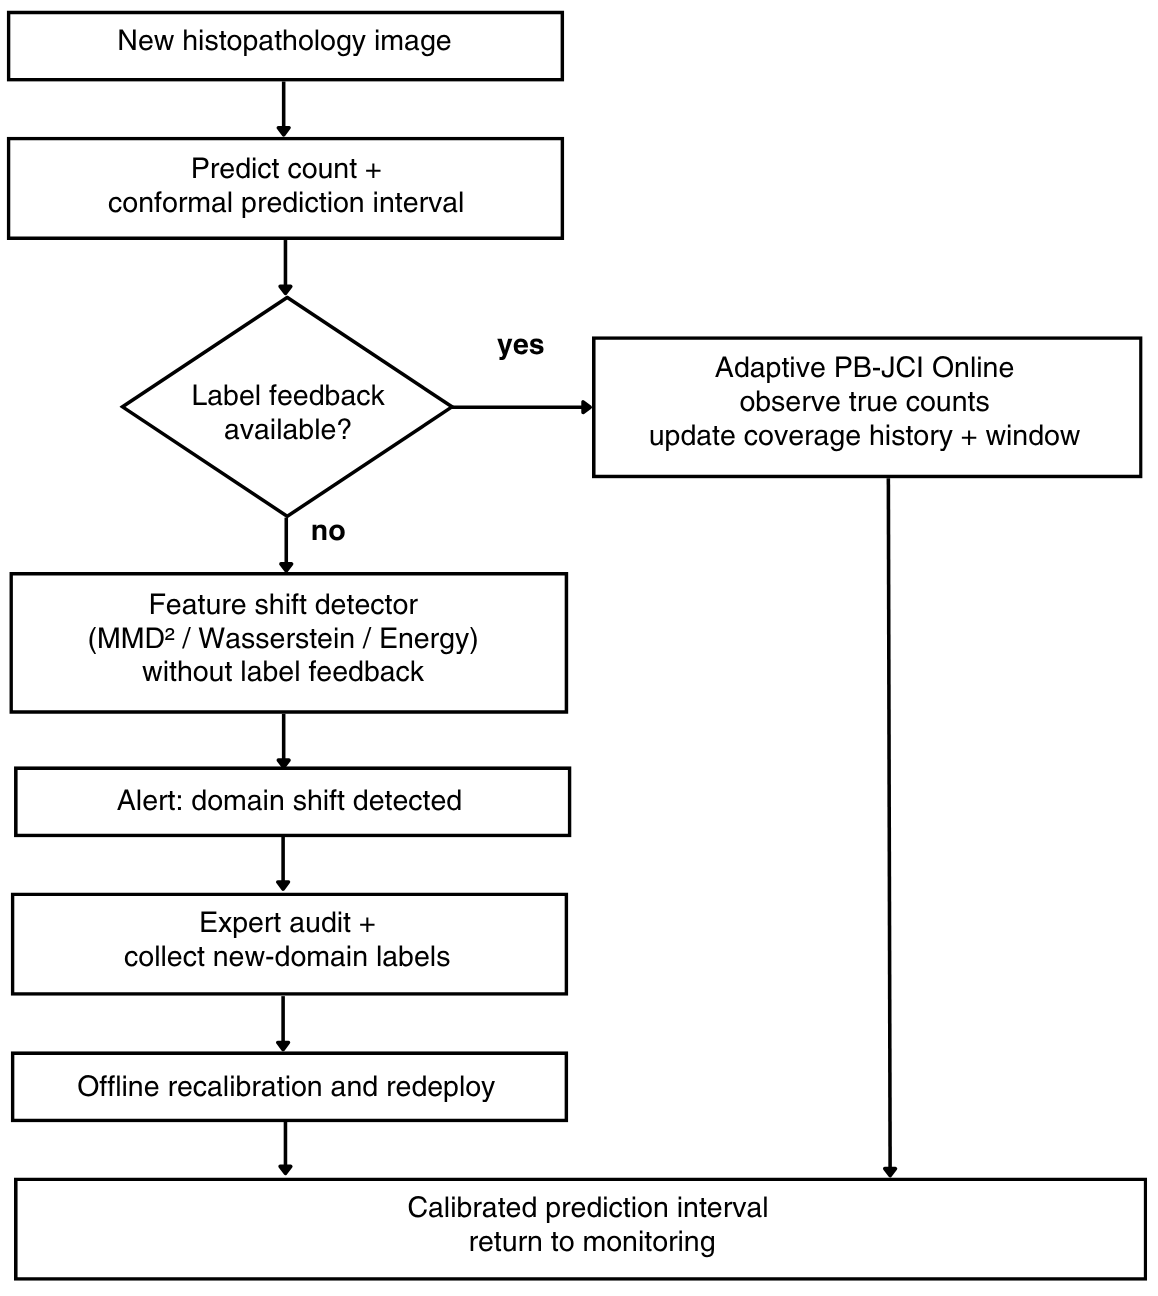
\includegraphics[width=0.95\textwidth]{F5_deployment_flow.png}
\caption{Deployment lifecycle of Adaptive PB-JCI Online in two regimes: online updating when label
feedback is available, and shift alerting for offline recalibration when labels are
unavailable.}\label{fig:deploy}
\end{figure}

%==============================================================================
\section{Experiments}\label{sec:exp}
%==============================================================================

\subsection{Setup}\label{sec:setup}

\textbf{Datasets.}
Chúng tôi đánh giá phương pháp trên ba bộ dữ liệu nhân tế bào nhuộm H\&E: PanNuke,
NuInsSeg và MoNuSAC. PanNuke được sử dụng làm bộ dữ liệu chính cho thí nghiệm đếm đa
lớp với \(K=5\). Theo cấu trúc ba fold của PanNuke, Fold~1 và Fold~2 được dùng để
huấn luyện hoặc tinh chỉnh các thành phần dự báo, trong khi Fold~3 được giữ cho đánh
giá conformal. Với mỗi calibration seed, dữ liệu đánh giá được chia ngẫu nhiên theo
tỉ lệ \(50/50\) thành tập hiệu chỉnh và tập kiểm thử. Tập hiệu chỉnh chỉ được dùng để
ước lượng ngưỡng conformal.

Đối với SAM3, chúng tôi đánh giá trên toàn bộ Fold~3 của PanNuke, gồm \(2{,}722\) ảnh
với \(n_{\mathrm{cal}}=n_{\mathrm{test}}=1{,}361\) cho mỗi seed. Đối với PathoSAM, để
tránh khả năng trùng lặp với dữ liệu huấn luyện, chúng tôi loại \(494\) ảnh mô đại
tràng khỏi Fold~3. Cụ thể, Lizard là một trong các bộ dữ liệu huấn luyện PathoSAM, tổng
hợp ảnh từ nhiều nguồn mô đại tràng và có thể chứa các ảnh thuộc phần colon của
PanNuke Fold~3. Do đó, PathoSAM được đánh giá trên tập con gồm \(2{,}228\) ảnh,
với \(n_{\mathrm{cal}}=n_{\mathrm{test}}=1{,}114\) cho mỗi seed.

NuInsSeg được dùng cho thí nghiệm dịch chuyển chéo bộ dữ liệu trong bài toán đếm tổng
số tế bào, tức \(K=1\). Trong thiết lập này, bộ hiệu chỉnh ban đầu đến từ PanNuke, còn
NuInsSeg được xem như luồng dữ liệu triển khai để đánh giá khả năng thích nghi trực
tuyến. MoNuSAC được dùng để kiểm tra khả năng tổng quát của cơ chế phủ đồng thời trong
thiết lập đếm đa lớp với số lớp khác PanNuke, cụ thể \(K=4\). Bảng~\ref{tab:data_split}
tóm tắt các bộ dữ liệu, thiết lập đánh giá và thống kê số nhân tế bào.
\begin{table}[t]
\caption{Summary of datasets, evaluation settings, and nuclei statistics. For
PanNuke Fold-3, the \#Images/\#Nuclei columns correspond to the \(2{,}228\)-image subset
used for PathoSAM (after removing \(494\) colon images); SAM3 is evaluated on all
\(2{,}722\) Fold-3 images.}
\label{tab:data_split}
\centering
\small
\setlength{\tabcolsep}{4pt}
\begin{tabularx}{\textwidth}{@{}LlclLcc@{}}
\toprule
Dataset & Task & \(K\) & Train & Cal/Test & \#Images & \#Nuclei \\
\midrule
PanNuke (Fold-3, subset) & multi-class counting & 5 & Fold~1+2 & Fold~3 (\(50/50\)) & \(2{,}228\) & \(54{,}835\) \\
NuInsSeg & total counting & 1 & - & PanNuke cal \(\to\) stream & \(665\) & \(35{,}138\) \\
MoNuSAC (test) & multi-class counting & 4 & train split & cal/test split & \(96\) & \(15{,}997\) \\
\botrule
\end{tabularx}
\end{table}

\textbf{Predictors and type head.}
Chúng tôi sử dụng hai backbone phân vùng và phát hiện khác nhau để kiểm tra mức độ phụ
thuộc của tầng hiệu chỉnh conformal vào kiến trúc dự báo. Backbone thứ nhất là
SAM3~\cite{carion2025sam3}, được tinh chỉnh bằng LoRA~\cite{hu2022lora} trên decoder;
backbone thứ hai là PathoSAM~\cite{archit2025patho}, một mô hình chuyên biệt cho phân
vùng nhân tế bào trong ảnh mô bệnh học. Sau giai đoạn huấn luyện hoặc tinh chỉnh ban
đầu, các backbone được cố định trong toàn bộ thí nghiệm conformal.

Với mỗi thực thể phát hiện, backbone cung cấp điểm objectness \(s_i\). Để ước lượng
xác suất lớp \(p_{ik}\), chúng tôi áp dụng một type head lên đặc trưng của từng thực
thể, thu được bằng cách gộp đặc trưng trong vùng mặt nạ tương ứng. Trong thực nghiệm,
type head là một MLP hai tầng, xuất phân phối softmax trên \(K\) lớp. Type head được
huấn luyện trên dữ liệu huấn luyện tương ứng bằng class-weighted cross-entropy loss để
xử lý mất cân bằng lớp, sau đó được cố định trong giai đoạn hiệu chỉnh. Tầng conformal chỉ sử dụng các đầu ra
\((s_i,p_{ik})\) cùng nhãn số đếm trên tập hiệu chỉnh.

\textbf{Distribution-shift scenarios.}
Chúng tôi đánh giá bốn kịch bản dịch chuyển có kiểm soát trên PanNuke: trong miền,
dịch chuyển nhẹ, dịch chuyển nặng và trôi phân phối theo thời gian. Trong kịch bản
trong miền, dữ liệu kiểm thử có cùng miền với tập hiệu chỉnh. Chúng tôi khảo sát các
biến đổi màu và hình thái ảnh gồm HED, HSV jitter và Gaussian blur ở nhiều mức cường
độ; trong các thí nghiệm chính, mức dịch chuyển nhẹ được đại diện bằng HSV jitter, còn
mức dịch chuyển nặng được đại diện bằng Gaussian blur. Trong kịch bản drift, luồng kiểm
thử được sắp xếp theo mức độ dịch chuyển tăng dần, từ trong miền sang nhẹ và nặng,
nhằm mô phỏng phân phối thay đổi theo thời gian.

Mức độ dịch chuyển của các biến đổi được định lượng bằng MMD\(^2\), Wasserstein-1 và
Energy distance trong Appendix~\ref{secA:shift}. Kết quả cho thấy độ lệch đặc trưng
tăng theo cường độ biến đổi, trong khi khác biệt giữa các fold của PanNuke là rất nhỏ.


\textbf{Baselines.}
\emph{Marginal Split} hiệu chỉnh từng lớp ở mức \(\alpha\), chỉ bảo đảm phủ biên cho
mỗi lớp mà không hiệu chỉnh cho phủ đồng thời. \emph{PB-JCI Split} là phiên bản tĩnh của phương pháp đề xuất, sử
dụng thang Poisson-Binomial và thống kê cực đại nhưng giữ ngưỡng conformal cố định.
\emph{PB-JCI Online-Fixed} sử dụng cùng điểm bất hợp lệ đồng thời nhưng cập nhật ngưỡng
bằng cửa sổ trượt cố định. \emph{Class-Strat Bonferroni} hiệu chỉnh riêng từng lớp với
mức lỗi được phân bổ theo hiệu chỉnh Bonferroni. Trong kịch bản chéo bộ dữ liệu, chúng tôi so sánh
thêm với các phương pháp conformal trực tuyến hiện đại gồm ACI, NexCP, FACI, SAOCP,
COP và Rolling-Origin CP.

Trừ khi có ghi chú khác, tất cả các phương pháp trực tuyến được khởi tạo từ cùng bộ
đệm hiệu chỉnh ban đầu, xử lý cùng thứ tự luồng dữ liệu, và nhận nhãn phản hồi sau khi
dự đoán tại cùng thời điểm. Thiết lập này giúp quy sự khác biệt về kết quả chủ yếu cho
cơ chế hiệu chỉnh, thay vì cho lượng thông tin được sử dụng. Quy tắc cập nhật ngưỡng
của các baseline conformal trực tuyến được tóm tắt trong Appendix~\ref{secA:baselines}.

\textbf{Metrics.}
Độ đo chính là coverage đồng thời. Với ảnh \(t\), dự đoán được xem là phủ đúng nếu
\(N_{t,k}\in \mathcal{C}_{t,k}\) với mọi lớp \(k=1,\dots,K\). Coverage được tính bằng
tỉ lệ các ảnh thỏa điều kiện này. Chúng tôi cũng báo cáo average width, được tính là
độ rộng trung bình của các khoảng trên các lớp và trên các ảnh. Vì average width có
thể bị chi phối bởi một số ít khoảng rất rộng, trong kịch bản dịch chuyển chéo bộ dữ
liệu, nơi phân phối độ rộng bị lệch mạnh, chúng tôi bổ sung median width, tức trung vị
độ rộng khoảng, như một thước đo bền hơn cho độ rộng điển hình.
Trong bài toán \(K=1\), width tương ứng với độ rộng khoảng dự đoán cho tổng số tế bào.

Bên cạnh coverage và width, chúng tôi sử dụng điểm Winkler, còn gọi là interval
score~\cite{winkler1972decision}, để đánh giá đồng thời độ hẹp và độ tin cậy của
khoảng dự đoán:
\begin{equation}
\mathrm{WS}_{\alpha}(\ell,u;y)
=
(u-\ell)
+
\frac{2}{\alpha}(\ell-y)\mathbf{1}\{y<\ell\}
+
\frac{2}{\alpha}(y-u)\mathbf{1}\{y>u\}.
\end{equation}
Điểm Winkler bằng width khi giá trị thật nằm trong khoảng và cộng thêm hình phạt khi
khoảng không phủ giá trị thật. Vì vậy, điểm thấp hơn thể hiện sự cân bằng tốt hơn giữa
coverage và độ hẹp của khoảng. Trong mỗi lần chạy, coverage là tỉ lệ ảnh được phủ đồng
thời, còn average width và Winkler được tính trung bình trên các lớp và các ảnh. Cả ba
độ đo sau đó được tổng hợp thành trung bình \(\pm\) độ lệch chuẩn qua các seed như báo
cáo trong từng bảng.

Trong các thí nghiệm trực tuyến, chúng tôi còn báo cáo coverage cục bộ và width cục
bộ trên cửa sổ trượt \(W_\ell=50\) để phân tích động học quanh thời điểm dịch chuyển.

\textbf{Implementation details.}
Mỗi cấu hình được chạy với nhiều seed hiệu chỉnh hoặc seed luồng, như ghi trong từng
bảng kết quả. Với SAM3, chúng tôi báo cáo trung bình và độ lệch chuẩn trên 15 lần chạy,
gồm 3 model seed và 5 calibration seed; với PathoSAM, kết quả được báo cáo trên 5
calibration seed. Trong thí nghiệm chéo bộ dữ liệu, các phương pháp trực tuyến được
đánh giá trên 5 stream seed. Các bảng trình bày trung bình \(\pm\) độ lệch chuẩn, trừ
các baseline tất định không phụ thuộc vào thứ tự luồng. Chi tiết siêu tham số huấn
luyện và cấu hình conformal được liệt kê trong Appendix~\ref{secA:impl}.

\textbf{Evaluation design.}
Thiết kế thực nghiệm của chúng tôi tách riêng hai vai trò chính của khung đề xuất.
Thành phần Poisson-Binomial kết hợp với thống kê cực đại chịu trách nhiệm cho phủ đồng
thời trong bài toán đếm đa lớp, và được đánh giá trên các bộ dữ liệu có taxonomy lớp xác
định như PanNuke và MoNuSAC. Ngược lại, cơ chế cửa sổ thích nghi được thiết kế cho các
kịch bản dịch chuyển trực tuyến nghiêm trọng, trong đó các điểm bất hợp lệ gần đây có
thể phản ánh miền dữ liệu hiện hành tốt hơn tập hiệu chỉnh ban đầu.
Vì các dịch chuyển có kiểm soát trên PanNuke vẫn nằm trong cùng bộ dữ liệu và cùng
taxonomy, chúng tôi sử dụng PB-JCI Online-Fixed để cô lập tác động của cập nhật bằng
cửa sổ trượt. Phiên bản đầy đủ, Adaptive PB-JCI Online, được đánh giá trong kịch bản
dịch chuyển chéo bộ dữ liệu PanNuke \(\to\) NuInsSeg. Do taxonomy giữa hai bộ dữ
liệu không tương thích, bài toán trong thiết lập này được quy về đếm tổng số tế bào,
tức \(K=1\).

\subsection{Conformal Counting under Controlled Shift}\label{sec:main}

Bảng~\ref{tab:main} đánh giá conformal counting đồng thời dưới bốn chế độ dịch chuyển có
kiểm soát trên PanNuke. Thí nghiệm nhằm kiểm tra ba khía cạnh: (i) liệu PB-JCI có đạt
joint coverage mục tiêu trong miền hay không; (ii) mức độ suy giảm của hiệu chỉnh tĩnh
khi dịch chuyển tăng từ nhẹ đến nặng, so với các biến thể cập nhật trực tuyến; và
(iii) tính nhất quán của xu hướng này trên hai backbone khác biệt, SAM3 và PathoSAM.

\begin{table}[!htbp]
\caption{Joint conformal counting under controlled shift on two backbones.
Each cell reports Coverage~\% (top) and Width (bottom) as mean \(\pm\) standard
deviation; the target coverage is 90\%. Bold rows mark the proposed variant (PB-JCI
Online-Fixed), not necessarily the best result.}
\label{tab:main}
\centering
\scriptsize
\setlength{\tabcolsep}{2.5pt}
\renewcommand{\arraystretch}{1.15}
\begin{tabularx}{\textwidth}{@{}p{0.23\textwidth}YYYY@{}}
\toprule
Method & In-dist & Mild & Severe & Drift \\
\midrule
\multicolumn{5}{@{}l}{\textit{(a) Backbone: SAM3 (LoRA)}}\\[2pt]
Marginal Split
& \makecell{62.7$\pm$1.6\\9.63$\pm$0.57}
& \makecell{54.8$\pm$1.9\\10.01$\pm$0.62}
& \makecell{61.8$\pm$2.0\\9.19$\pm$0.41}
& \makecell{59.9$\pm$1.5\\9.60$\pm$0.54} \\

ACI
& \makecell{89.9$\pm$0.1\\14.62$\pm$0.79}
& \makecell{89.7$\pm$0.1\\18.70$\pm$1.41}
& \makecell{89.3$\pm$0.2\\24.54$\pm$1.42}
& \makecell{89.4$\pm$0.1\\19.45$\pm$1.24} \\

PB-JCI Split
& \makecell{90.0$\pm$1.3\\13.54$\pm$0.74}
& \makecell{82.9$\pm$1.2\\13.93$\pm$0.80}
& \makecell{81.1$\pm$2.2\\12.79$\pm$0.53}
& \makecell{84.8$\pm$1.0\\13.41$\pm$0.70} \\

\textbf{PB-JCI Online-Fixed}
& \makecell{\textbf{90.5$\pm$0.3}\\\textbf{13.76$\pm$0.74}}
& \makecell{\textbf{89.9$\pm$0.3}\\\textbf{16.18$\pm$0.88}}
& \makecell{\textbf{89.4$\pm$0.4}\\\textbf{17.77$\pm$0.34}}
& \makecell{\textbf{89.3$\pm$0.4}\\\textbf{15.56$\pm$0.59}} \\

Class-Strat Bonferroni
& \makecell{94.4$\pm$1.1\\18.59$\pm$0.69}
& \makecell{89.2$\pm$1.5\\19.05$\pm$0.78}
& \makecell{85.3$\pm$1.8\\16.19$\pm$0.41}
& \makecell{89.9$\pm$1.1\\17.91$\pm$0.62} \\
\midrule
\multicolumn{5}{@{}l}{\textit{(b) Backbone: PathoSAM}}\\[2pt]
Marginal Split
& \makecell{65.1$\pm$1.9\\8.84$\pm$0.14}
& \makecell{57.6$\pm$1.8\\8.93$\pm$0.13}
& \makecell{17.3$\pm$0.7\\6.98$\pm$0.09}
& \makecell{46.4$\pm$1.2\\8.28$\pm$0.16} \\

ACI
& \makecell{89.9$\pm$0.1\\14.79$\pm$0.58}
& \makecell{89.6$\pm$0.1\\18.05$\pm$0.57}
& \makecell{87.4$\pm$0.3\\68.70$\pm$2.36}
& \makecell{87.2$\pm$0.3\\32.76$\pm$1.64} \\

PB-JCI Split
& \makecell{89.7$\pm$1.0\\13.67$\pm$0.19}
& \makecell{83.8$\pm$1.3\\13.75$\pm$0.22}
& \makecell{35.7$\pm$1.2\\11.38$\pm$0.17}
& \makecell{70.1$\pm$1.1\\12.98$\pm$0.24} \\

\textbf{PB-JCI Online-Fixed}
& \makecell{\textbf{90.4$\pm$0.2}\\\textbf{13.94$\pm$0.33}}
& \makecell{\textbf{89.2$\pm$0.4}\\\textbf{15.87$\pm$0.13}}
& \makecell{\textbf{85.7$\pm$0.4}\\\textbf{54.02$\pm$0.52}}
& \makecell{\textbf{85.6$\pm$0.5}\\\textbf{23.87$\pm$0.45}} \\

Class-Strat Bonferroni
& \makecell{96.6$\pm$0.5\\20.17$\pm$0.64}
& \makecell{93.7$\pm$0.7\\20.20$\pm$0.66}
& \makecell{48.5$\pm$1.7\\16.54$\pm$0.73}
& \makecell{79.6$\pm$0.8\\19.05$\pm$0.68} \\
\botrule
\end{tabularx}
\end{table}

Trên SAM3 (khối a), hiệu chỉnh tĩnh không đủ dưới dịch chuyển: Marginal Split chỉ
đạt \(54.8\)--\(62.7\%\) coverage, trong khi PB-JCI Split suy giảm từ \(90.0\%\) trong
miền xuống \(81.1\%\) ở chế độ nặng. ACI duy trì coverage gần mục tiêu
\((\approx 89\%)\) nhưng width tăng mạnh, đạt \(24.54\) ở chế độ nặng. Ngược lại,
PB-JCI Online-Fixed giữ coverage quanh \(89\)-\(90\%\) ở mọi chế độ và tạo khoảng hẹp
hơn ACI rõ rệt; ở chế độ nặng, width giảm từ \(24.54\) xuống \(17.77\), tương đương
hẹp hơn khoảng \(28\%\). Class-Strat Bonferroni thường phủ dư và tạo khoảng rộng, cho
thấy nhược điểm của việc hiệu chỉnh độc lập từng lớp.

Xu hướng cải thiện tương tự xuất hiện trên PathoSAM (khối b), một backbone khác với
SAM3. PB-JCI Split suy giảm mạnh dưới dịch chuyển nặng, chỉ còn \(35.7\%\) coverage,
trong khi PB-JCI Online-Fixed nâng coverage lên \(85.7\%\) và vẫn tạo khoảng hẹp hơn
ACI \((54.02\) so với \(68.70)\). Tuy nhiên, do PathoSAM có xu hướng quá tự tin, dẫn
đến \(\sigma_k\) nhỏ, cửa sổ cố định chưa khôi phục hoàn toàn coverage về mức mục tiêu
trong kịch bản nặng. Kết quả trên hai backbone cho thấy tầng conformal mang lại cải
thiện đáng kể bên cạnh lựa chọn kiến trúc dự báo. Đồng thời, hạn chế của cửa sổ cố
định dưới dịch chuyển mạnh trên PathoSAM là động lực trực tiếp cho phiên bản đầy đủ
Adaptive PB-JCI Online, được đánh giá ở Section~\ref{sec:cross}.

\subsection{Cross-Dataset Shift and Online Conformal Baselines}\label{sec:cross}

Trong phần này, chúng tôi đánh giá một kịch bản dịch chuyển chéo bộ dữ liệu, trong đó
bộ hiệu chỉnh ban đầu đến từ PanNuke còn luồng triển khai đến từ NuInsSeg với backbone
PathoSAM. Đây là một thiết lập khó hơn các dịch chuyển có kiểm soát ở
Section~\ref{sec:main}, vì sai khác giữa nguồn và đích không chỉ đến từ các biến đổi
ảnh nhân tạo mà còn từ khác biệt về bộ dữ liệu, cơ quan, quy trình chú giải và đặc
tính hình ảnh. Trong kịch bản NuInsSeg, bài toán được gộp về đếm tổng số tế bào
(\(K=1\)). Do đó, mọi baseline trực tuyến được áp dụng trên cùng chuỗi điểm bất hợp lệ
vô hướng, được khởi tạo từ cùng bộ đệm hiệu chỉnh PanNuke và nhận cùng nhãn phản hồi
sau mỗi dự đoán.

\begin{table}[!ht]
\caption{Cross-dataset shift with PathoSAM in the PanNuke $\to$ NuInsSeg setting.
The target coverage is $90\%$; coverage and Winkler are reported as mean $\pm$ standard
deviation over 5 stream seeds. Lower Winkler is better.}
\label{tab:cross}
\centering
\begin{tabular}{@{}lcccc@{}}
\toprule
Method & Coverage (\%) & Avg. width & Med. width & Winkler $\downarrow$ \\
\midrule
ACI
& 84.0$\pm$0.2 & 63.58 & 50.50 & 129.55$\pm$3.78 \\
NexCP
& 84.7$\pm$0.6 & 55.52 & 50.84 & 119.56$\pm$1.29 \\
FACI
& 85.1$\pm$0.6 & 56.71 & 51.28 & 118.93$\pm$0.99 \\
SAOCP
& 87.8$\pm$0.5 & 61.32 & 54.70 & 113.63$\pm$1.53 \\
COP
& 87.9$\pm$0.2 & 60.60 & 54.91 & 113.13$\pm$2.00 \\
Rolling-Origin CP
& 89.5$\pm$0.7 & 64.39 & 58.19 & 110.24$\pm$2.54 \\
PB-JCI Online-Fixed
& 81.8$\pm$1.0 & 53.11 & 47.75 & 125.96$\pm$2.17 \\
\textbf{Adaptive PB-JCI Online}
& \textbf{90.0$\pm$0.6} & 66.50 & 60.02 & \textbf{108.67$\pm$2.94} \\
\botrule
\end{tabular}
\end{table}

Bảng~\ref{tab:cross} báo cáo coverage, average width, median width và điểm Winkler của
các phương pháp trong kịch bản này. Kết quả cho thấy các cơ chế bán thích nghi vẫn chưa
đủ để duy trì empirical coverage trong thiết lập dịch chuyển chéo bộ dữ liệu. PB-JCI
Online-Fixed cải thiện so với split tĩnh nhưng
chỉ đạt $81.8\pm1.0\%$, cho thấy cửa sổ cố định phản ứng chưa đủ nhanh khi phân phối
thay đổi mạnh. Các baseline conformal trực tuyến như ACI, NexCP và FACI đạt coverage
trong khoảng $84$--$85\%$, trong khi SAOCP, COP và Rolling-Origin CP tiến gần hơn
tới mục tiêu, đạt khoảng $87.8$--$89.5\%$.

Adaptive PB-JCI Online là phương pháp duy nhất đạt empirical coverage trung bình ở mức
danh nghĩa, với $90.0\pm0.6\%$. Cải thiện chính của phương pháp nằm ở khả năng phục hồi
empirical coverage dưới dịch chuyển chéo bộ dữ liệu, thay vì tạo ra khoảng hẹp hơn.
Cụ thể, average width của Adaptive PB-JCI Online là $66.50$, lớn hơn nhiều baseline,
phản ánh trade-off cần chấp nhận để đưa coverage về mục tiêu khi bộ dự báo ban đầu bị
lệch miền và có xu hướng quá tự tin. Tuy nhiên, median width của phương pháp là $60.02$,
gần với Rolling-Origin CP ($58.19$) và COP ($54.91$), cho thấy độ rộng điển hình
không tăng quá mức; phần tăng của average width chủ yếu đến từ một số ảnh khó cần
khoảng dự đoán rộng hơn.

Về điểm Winkler, Adaptive PB-JCI Online đạt giá trị thấp nhất
($108.67\pm2.94$). Dù khoảng cách so với Rolling-Origin CP
($110.24\pm2.54$) không lớn, phương pháp là biến thể duy nhất đưa coverage trung bình
về đúng mức mục tiêu. Kết quả này cho thấy cơ chế cửa sổ thích nghi chủ yếu giúp khép
lại khoảng hụt coverage của các baseline, đồng thời duy trì mức tăng width ở mức chấp
nhận được.

Động học này được minh họa trong Hình~\ref{fig:streaming}. Sau điểm đổi miền, coverage
cục bộ của các phương pháp tĩnh suy giảm rõ rệt, trong khi Adaptive PB-JCI Online điều
chỉnh ngưỡng để đưa coverage cục bộ trở lại gần mục tiêu. Đồng thời, width cục bộ tăng
ở vùng dữ liệu khó, cho thấy phương pháp chấp nhận đánh đổi độ hẹp để duy trì độ tin
cậy của khoảng dự đoán.

\begin{figure}[t]
\centering
\includegraphics[width=\textwidth]{F2_streaming_coverage.png}
\caption{Online dynamics under cross-dataset shift PanNuke $\to$ NuInsSeg with the
PathoSAM backbone. Quantities are computed over a sliding window of 50 steps:
\textbf{(a)} local coverage versus the 90\% target; \textbf{(b)} local width.}
\label{fig:streaming}
\end{figure}

\subsection{Ablation Study}\label{sec:ablation}

Để tách riêng vai trò của từng thành phần trong Adaptive PB-JCI Online, chúng tôi thực
hiện ablation dạng leave-one-out trên kịch bản dịch chuyển chéo bộ dữ liệu
PathoSAM: PanNuke \(\to\) NuInsSeg. Thiết lập này được chọn vì tạo ra sai khác phân
phối đủ lớn để làm rõ đóng góp của các thành phần thích nghi. Do NuInsSeg được sử dụng
cho bài toán đếm tổng số tế bào \((K=1)\), thí nghiệm tập trung đánh giá tầng hiệu
chỉnh conformal, thang chuẩn hóa Poisson-Binomial và cơ chế cửa sổ thích nghi trực
tuyến. Vai trò của thống kê cực đại đối với phủ đồng thời đa lớp được đánh giá riêng ở
cuối phần này.

\begin{table}[!htbp]
\caption{Leave-one-out ablation with target coverage $90\%$.
Each variant removes one component from the full model. Lower Winkler is better.}
\label{tab:ablation}
\centering
\small
\begin{tabular}{@{}lccc@{}}
\toprule
Variant & Coverage (\%) & Avg.\ width & Winkler $\downarrow$ \\
\midrule
Naive PB interval, no conformal       & $10.4$        & $4.19$  & $319.09$ \\
Full w/o online update (static split) & $41.5$        & $18.00$ & $226.44$ \\
Full w/o adaptive window (fixed)      & $81.8\pm1.0$  & $53.11$ & $125.96\pm2.17$ \\
Full w/o PB-$\sigma$ (raw residual)   & $90.0\pm0.5$  & $83.47$ & $156.37\pm2.08$ \\
\midrule
\textbf{Full Adaptive PB-JCI Online}  & $\mathbf{90.0\pm0.6}$ & $66.50$ & $\mathbf{108.67\pm2.94}$ \\
\botrule
\end{tabular}
\end{table}

Bảng~\ref{tab:ablation} cho thấy mỗi thành phần đóng một vai trò riêng trong hệ thống.
Nếu bỏ toàn bộ tầng conformal và chỉ dùng khoảng dựa trên phương sai
Poisson-Binomial, biến thể Naive PB interval chỉ đạt $10.4\%$ coverage dù average
width rất nhỏ $(4.19)$. Kết quả này cho thấy phương sai giải tích chỉ cung cấp một
thang bất định ban đầu, chưa đủ để tạo khoảng dự đoán đáng tin cậy; mức sai lệch thực
tế vẫn cần được hiệu chỉnh bằng conformal calibration.

Cập nhật trực tuyến là yếu tố then chốt dưới dịch chuyển chéo bộ dữ liệu. Khi thay
phương pháp đầy đủ bằng split conformal tĩnh, coverage chỉ đạt $41.5\%$, cho thấy
ngưỡng học từ miền nguồn PanNuke không còn phù hợp với miền đích NuInsSeg. Sử dụng cửa
sổ trực tuyến cố định cải thiện coverage lên $81.8\pm1.0\%$, nhưng vẫn chưa đạt mục
tiêu do cửa sổ cố định phản ứng chậm trước dịch chuyển mạnh. Ngược lại, cơ chế cửa sổ
thích nghi khôi phục coverage trung bình về $90.0\pm0.6\%$, cho thấy việc điều chỉnh
kích thước cửa sổ theo phản hồi coverage là cần thiết trong thiết lập này.

Thang PB-\(\sigma\) chủ yếu ảnh hưởng đến hiệu quả của khoảng dự đoán hơn là khả năng
đạt coverage. Khi bỏ PB-\(\sigma\) và dùng residual thô, phương pháp vẫn đạt coverage
$90.0\pm0.5\%$ nhờ cơ chế adaptive online, nhưng average width tăng từ $66.50$ lên
$83.47$, đồng thời Winkler tăng từ $108.67$ lên $156.37$. Điều này cho thấy
phương sai Poisson-Binomial giúp phân bổ độ rộng theo độ khó của từng ảnh, thay vì phải
nới rộng khoảng gần như đồng đều để bù cho các trường hợp khó.

Do NuInsSeg được quy về bài toán một lớp \((K=1)\), thống kê cực đại trong
Bảng~\ref{tab:ablation} trùng với điểm bất hợp lệ vô hướng và chưa kiểm tra được vai
trò của cơ chế phủ đồng thời đa lớp. Vì vậy, chúng tôi đánh giá riêng thành phần này
trên các thiết lập đa lớp. Trên PanNuke in-distribution (Bảng~\ref{tab:main}),
max-statistic đạt coverage $90.4\%$ với average width $13.94$; trong khi đó, hiệu chỉnh Bonferroni từng lớp
đẩy coverage lên $96.6\%$, tức phủ dư so với mục tiêu $90\%$, và làm average width
tăng lên $20.17$. Kết quả này cho thấy thống kê cực đại hiệu chỉnh trực tiếp cho sự
kiện phủ đồng thời của vector số đếm mà không bị quá bảo thủ như hiệu chỉnh độc lập
từng lớp. Khả năng tổng quát của cơ chế này sang số lớp khác được đánh giá trên
MoNuSAC \((K=4)\) ở Section~\ref{sec:monusac}.

\subsection{Generalization to a Different Number of Classes}\label{sec:monusac}

Các thí nghiệm chính trên PanNuke sử dụng \(K=5\) lớp, trong khi thí nghiệm chéo bộ
dữ liệu trên NuInsSeg được quy về bài toán một lớp \((K=1)\). Để đánh giá liệu cơ chế
phủ đồng thời dựa trên thống kê cực đại có phụ thuộc vào số lớp cụ thể của PanNuke hay
không, chúng tôi thực hiện thêm thí nghiệm trên MoNuSAC, bộ dữ liệu có \(K=4\) lớp
nhân tế bào. Thiết lập này cho phép kiểm tra khả năng tổng quát của PB-JCI trong một
bài toán đếm đa lớp với cấu trúc nhãn khác.

\begin{table}[t]
\caption{Generalization to a different number of classes on MoNuSAC (\(K=4\), target
joint coverage \(90\%\)).}
\label{tab:monusac}
\centering
\begin{tabular}{@{}lcc@{}}
\toprule
Method & Joint coverage (\%) & Avg.\ width \\
\midrule
Marginal Split & $82.9\pm5.2$ & $131.87$ \\
Class-Strat Bonferroni & $87.1\pm6.4$ & $170.33$ \\
PB-JCI Max-Statistic & $\mathbf{91.7\pm1.9}$ & $140.19$ \\
\botrule
\end{tabular}
\end{table}

Kết quả trong Bảng~\ref{tab:monusac} cho thấy hiệu chỉnh marginal không đủ để đảm bảo
phủ đồng thời: mặc dù từng lớp có thể đạt coverage tương đối cao, xác suất mọi lớp
được phủ cùng lúc chỉ đạt $82.9\pm5.2\%$, thấp hơn đáng kể so với mục tiêu \(90\%\).
Marginal Split cho average width nhỏ nhất ($131.87$), nhưng độ hẹp này đánh đổi bằng
việc không đạt phủ đồng thời, nên không phải là một so sánh có ý nghĩa ở cùng mức
độ tin cậy.
Class-Strat Bonferroni cải thiện một phần bằng cách hiệu chỉnh riêng từng lớp với mức
lỗi phân bổ, nhưng vẫn đạt coverage đồng thời thấp hơn mục tiêu
($87.1\pm6.4\%$) và tạo khoảng rộng hơn, với average width $170.33$. Độ lệch chuẩn lớn
của các baseline trên MoNuSAC (ví dụ $\pm6.4$ với Bonferroni) phản ánh kích thước tập
kiểm thử nhỏ ($96$ ảnh), khiến ước lượng empirical coverage biến động hơn so với
PanNuke.

Ngược lại, PB-JCI với thống kê cực đại đạt coverage đồng thời
$91.7\pm1.9\%$ và average width $140.19$. Kết quả này cho thấy max-statistic học trực
tiếp phân vị của sai số chuẩn hóa lớn nhất trên các lớp, nên phù hợp hơn với sự kiện
phủ đồng thời của toàn bộ vector số đếm. Việc đạt coverage trên MoNuSAC, nơi số lớp
khác với PanNuke, cho thấy cơ chế joint conformal không phụ thuộc vào số lớp cụ thể
của bộ dữ liệu chính.

Hai phân tích bổ sung trong Appendix tiếp tục củng cố kết quả chính. Thứ nhất, coverage
theo từng lớp trên PanNuke cho thấy không lớp nào bị under-cover, với mọi lớp đều đạt
trên \(94\%\) (Appendix~\ref{secA:perclass}). Thứ hai, khảo sát độ nhạy cho thấy phương
pháp bền với các siêu tham số, trong đó \(w_{\min}\) là tham số chính điều khiển tốc độ
thích nghi (Appendix~\ref{secA:sensitivity}).

%==============================================================================
\section{Conclusion}\label{sec:conclusion}

Chúng tôi đã trình bày Adaptive PB-JCI Online, một khung conformal nhằm định lượng độ
bất định cho bài toán đếm tế bào đa lớp trên ảnh mô bệnh học. Thay vì thay đổi kiến
trúc phân vùng hoặc tối ưu lại bộ phát hiện, phương pháp bổ sung một tầng hiệu chỉnh
nhẹ lên trên các backbone sẵn có. Tầng này kết hợp ba thành phần: phương sai giải tích
từ phân phối Poisson-Binomial để chuẩn hóa điểm bất hợp lệ, thống kê cực đại để xây
dựng khoảng dự đoán phủ đồng thời cho vector số đếm đa lớp, và cơ chế hiệu chỉnh trực
tuyến với kích thước cửa sổ thích nghi theo phản hồi coverage.

Thực nghiệm trên ba bộ dữ liệu và hai backbone cho thấy các bộ hiệu chỉnh tĩnh có thể
suy giảm mạnh khi phân phối dữ liệu thay đổi, trong khi các biến thể trực tuyến cải
thiện đáng kể empirical coverage dưới dịch chuyển. Trong các kịch bản dịch chuyển có
kiểm soát, PB-JCI Online-Fixed duy trì empirical coverage gần mức mục tiêu trên SAM3 và
cải thiện rõ rệt coverage trên PathoSAM, dù vẫn còn under-cover dưới dịch chuyển mạnh. Trong kịch bản
dịch chuyển chéo bộ dữ liệu nghiêm trọng, Adaptive PB-JCI Online khôi phục empirical
coverage trung bình về \(90.0\pm0.6\%\) và đạt điểm Winkler thấp nhất trong các
phương pháp so sánh. Kết quả ablation cho thấy cập nhật trực tuyến và cửa sổ thích
nghi là các yếu tố chính để phục hồi coverage, trong khi thang Poisson-Binomial giúp
tăng hiệu quả của khoảng dự đoán. Thí nghiệm trên MoNuSAC với \(K=4\) cũng cho thấy
thống kê cực đại có thể tổng quát sang số lớp khác và hiệu chỉnh trực tiếp cho sự kiện
phủ đồng thời.

Nhìn chung, kết quả cho thấy một tầng conformal nhẹ, độc lập với backbone, có thể bổ
sung khoảng dự đoán đáng tin cậy cho các hệ thống đếm tế bào hiện có, đặc biệt trong
các điều kiện triển khai có dịch chuyển phân phối.

\textbf{Limitations and future work.}
Phương pháp hiện tại giả định rằng nhãn đếm thật được quan sát sau dự đoán để cập nhật
coverage và điểm bất hợp lệ. Trong các triển khai không có nhãn phản hồi, hệ thống
không thể tự hiệu chỉnh trực tuyến; thay vào đó, các tín hiệu phát hiện dịch chuyển
chỉ có thể được dùng để kích hoạt rà soát và hiệu chỉnh lại ngoại tuyến. Ngoài ra, các
bảo đảm hữu hạn mẫu của split conformal chỉ áp dụng trực tiếp dưới giả định trao đổi
được. Dưới dịch chuyển phân phối, kết quả của chúng tôi nên được hiểu là đánh giá thực
nghiệm về khả năng phục hồi coverage, thay vì một bảo đảm lý thuyết mới cho dịch
chuyển tùy ý.

Phương pháp cũng phụ thuộc vào chất lượng của điểm objectness và xác suất lớp do
backbone và type head cung cấp, đặc biệt khi các đầu ra này quá tự tin hoặc bị lệch
miền. Trong tương lai, chúng tôi sẽ mở rộng khung đề xuất cho các chế độ phản hồi thưa
hoặc trễ, cải thiện hiệu chỉnh khi bộ dự báo bị miscalibration mạnh, và đánh giá trên
các luồng dữ liệu lâm sàng thực tế. Cuối cùng, phương pháp được thiết kế để hỗ trợ định
lượng độ bất định trong nghiên cứu và chưa được kiểm định cho chẩn đoán lâm sàng.

%==============================================================================
\begin{appendices}

\section{Implementation Details}\label{secA:impl}

Bảng~\ref{tab:impl} liệt kê cấu hình huấn luyện backbone, type head và tầng conformal.
Backbone được đóng băng trong toàn bộ quá trình hiệu chỉnh conformal; chỉ type head
và (với SAM3) các trọng số LoRA được huấn luyện trước.
\begin{table}[htbp]
\caption{Implementation details.}
\label{tab:impl}
\centering
\small
\begin{tabular}{@{}ll@{}}
\toprule
Component & Configuration \\
\midrule
Backbone 1 & SAM3, decoder fine-tuned with LoRA (FFN-only) \\
\quad LoRA & rank $r=16$, $\alpha=32$, dropout $0.05$; $\sim\!0.44$M parameters ($\approx 0.05\%$) \\
\quad LoRA training & AdamW, lr $3\times10^{-4}$, weight decay $10^{-4}$, warmup $500$ steps, $2$ epochs, $3$ model seeds \\
Backbone 2 & PathoSAM (generalist, fully frozen) \\
Type head & MLP: Linear$(256\!\to\!128)$-LayerNorm-ReLU-Dropout$(0.1)$-Linear$(128\!\to\!K)$ \\
\quad Type head training & Adam, lr $10^{-3}$, weight decay $10^{-4}$, batch $512$, $60$ epochs, class-weighted cross-entropy \\
Conformal & $\alpha=0.1$; base window $W=300$ \\
\quad Adaptive & $w_{\min}=40$, $w_{\max}=300$, $m=50$, $\rho_s=0.9$, $\rho_g=1.05$, $\beta=0.03$ \\
\botrule
\end{tabular}
\end{table}

\section{Distribution Shift Magnitudes}\label{secA:shift}

Bảng~\ref{tab:shift} định lượng mức độ dịch chuyển của các biến đổi có kiểm soát trên
PanNuke bằng khoảng cách đặc trưng giữa tập tham chiếu Fold~1 và các điều kiện kiểm
thử, trung bình qua 5 seed. Chúng tôi khảo sát HED, Gaussian blur và HSV jitter ở hai
mức cường độ để kiểm tra độ lệch đặc trưng do từng loại biến đổi tạo ra. Trong các thí
nghiệm chính, HSV jitter được dùng làm đại diện cho dịch chuyển nhẹ, còn Gaussian blur
được dùng làm đại diện cho dịch chuyển nặng. Kết quả cho thấy các khoảng cách đặc
trưng tăng theo cường độ biến đổi, trong khi khác biệt giữa các fold trong PanNuke gần
như bằng không.
\begin{table}[htbp]
\caption{Distribution shift magnitudes measured by feature distances (averaged over
5 seeds).}
\label{tab:shift}
\centering
\begin{tabular}{@{}lccc@{}}
\toprule
Condition & MMD$^2$ & Wasserstein-1 & Energy \\
\midrule
Within-PanNuke fold2/3
& 0.0000-0.0001 & 0.0120-0.0122 & 0.0286-0.0292 \\
HED mild $\to$ severe
& 0.0253 $\to$ 0.1177 & 0.0382 $\to$ 0.0889 & 0.0914 $\to$ 0.2014 \\
Blur mild $\to$ severe
& 0.0026 $\to$ 0.1855 & 0.0151 $\to$ 0.0942 & 0.0390 $\to$ 0.2234 \\
HSV mild $\to$ severe
& 0.0000 $\to$ 0.0342 & 0.0065 $\to$ 0.0440 & 0.0170 $\to$ 0.1060 \\
\botrule
\end{tabular}
\end{table}

\section{Baseline Update Rules}\label{secA:baselines}

Bảng~\ref{tab:baselines} tóm tắt quy tắc cập nhật ngưỡng của các baseline conformal
trực tuyến trong kịch bản chéo bộ dữ liệu. Tất cả các phương pháp được áp dụng trên
cùng chuỗi điểm bất hợp lệ vô hướng, khởi tạo từ cùng bộ đệm hiệu chỉnh PanNuke.

\begin{table}[htbp]
\caption{Update rules of the online conformal baselines.
\(\mathrm{err}_t\) is the miscoverage indicator at step \(t\), \(s\) is the
nonconformity score, and \(\hat{F}\) is the empirical CDF over the window.}
\label{tab:baselines}
\centering
\small
\begin{tabularx}{\textwidth}{@{}lX@{}}
\toprule
Method & Threshold update \\
\midrule
ACI~\cite{gibbs2021adaptive}
& Update the error level via
\(\alpha_{t+1}=\alpha_t+\gamma(\alpha-\mathrm{err}_t)\), then take the
\((1-\alpha_t)\)-quantile; \(\gamma=0.05\). \\

NexCP~\cite{barber2023conformal}
& Take a time-decayed weighted quantile with
\(w_i=\rho^{\,t-i}\) over the nonconformity history; \(\rho=0.99\). \\

FACI~\cite{gibbs2024conformal}
& Aggregate multiple ACI experts with different \(\gamma\) values via exponential
weights based on the pinball loss. \\

SAOCP~\cite{bhatnagar2023improved}
& Update via strongly adaptive online learning over an expert set across multiple
time scales. \\

COP~\cite{hu2026conformal}
& Update a preliminary threshold via
\(\hat{q}\leftarrow \hat{q}+\eta(\mathbf{1}[s>\hat{q}]-\alpha)\), then correct via
\(q=\hat{q}-\lambda(\hat{F}(\hat{q})-(1-\alpha))\); \(\eta=5,\lambda=1\). \\

Rolling-Origin CP~\cite{halkiewicz2026rolling}
& Use volatility-normalized conformal and select the window size via offline
Winkler cross-validation. \\
\botrule
\end{tabularx}
\end{table}
\section{Per-Class Coverage}\label{secA:perclass}

Vì coverage đồng thời được tính trên toàn bộ vector số đếm, chúng tôi kiểm tra thêm
coverage theo từng lớp để đánh giá liệu có lớp nào bị phủ thiếu một cách hệ thống hay
không, đặc biệt khi PanNuke có phân bố lớp mất cân bằng mạnh. Bảng~\ref{tab:perclass}
báo cáo coverage và width theo từng lớp của PB-JCI Online-Fixed trên PanNuke
in-distribution. Mọi lớp đều đạt coverage ít nhất \(94\%\) khi coverage đồng thời là
\(90.5\%\), cho thấy không có lớp nào bị phủ thiếu. Lớp Neoplastic có coverage biên
thấp nhất \((94.4\%)\) và width lớn nhất \((24.08)\), phù hợp với việc đây là lớp phổ
biến và khó hơn. Ngược lại, lớp hiếm Dead được phủ với khoảng rất hẹp \((2.03)\),
tương ứng với số đếm nhỏ hơn. Kết quả này cho thấy thang \(\sigma_k\) giúp phân bổ độ
rộng theo mức độ khó và mật độ của từng lớp, thay vì nới rộng khoảng một cách đồng đều.

\begin{table}[htbp]
\caption{Per-class coverage and width of PB-JCI Online-Fixed on PanNuke
in-distribution with the SAM3 backbone. The corresponding joint coverage is $90.5\%$.}
\label{tab:perclass}
\centering
\small
\begin{tabular}{@{}lcc@{}}
\toprule
Class & Coverage (\%) & Width \\
\midrule
Neoplastic   & 94.4 & 24.08 \\
Inflammatory & 99.7 & 12.18 \\
Connective   & 98.7 & 21.27 \\
Dead         & 98.1 & 2.03 \\
Epithelial   & 98.2 & 9.24 \\
\botrule
\end{tabular}
\end{table}

\section{Hyperparameter Sensitivity}\label{secA:sensitivity}

Bảng~\ref{tab:sensitivity} khảo sát độ nhạy của Adaptive PB-JCI Online với ba siêu
tham số cửa sổ trên kịch bản chéo bộ dữ liệu. Phương pháp khá ổn định với cận trên
$w_{\max}$ và cửa sổ đo coverage $m$: coverage lần lượt nằm trong khoảng
$89.7$--$90.1\%$ và $90.0$--$90.2\%$, trong khi Winkler chỉ dao động nhỏ trên các giá
trị khảo sát. Siêu tham số có ảnh hưởng rõ nhất là cận dưới $w_{\min}$, đóng vai trò
điều khiển tốc độ thích nghi. Khi $w_{\min}$ nhỏ, phương pháp phản ứng nhanh hơn và đạt
coverage cao hơn nhưng tạo khoảng rộng hơn, ví dụ $w_{\min}=20$ cho $91.2\%$ coverage
và width $74.09$. Ngược lại, $w_{\min}$ lớn làm thích nghi chậm hơn và dẫn đến phủ
thiếu, với $w_{\min}=80$ chỉ đạt $88.2\%$ coverage. Cấu hình mặc định
$(w_{\min},w_{\max},m)=(40,300,50)$ đạt đúng mục tiêu $90\%$ và nằm trong vùng Winkler
thấp, cho thấy phương pháp không đòi hỏi tinh chỉnh siêu tham số tỉ mỉ.

\begin{table}[htbp]
\caption{Sensitivity of Adaptive PB-JCI Online to the window hyperparameters in the
PathoSAM $\to$ NuInsSeg setting. Each group varies one hyperparameter around the
default configuration (bold); lower Winkler is better.}
\label{tab:sensitivity}
\centering
\small
\begin{tabular}{@{}llccc@{}}
\toprule
Parameter & Value & Coverage (\%) & Width & Winkler $\downarrow$ \\
\midrule
$w_{\min}$ & 20 & 91.2$\pm$0.4 & 74.09 & 109.50 \\
$w_{\min}$ & \textbf{40} & 90.0$\pm$0.6 & 66.50 & 108.67 \\
$w_{\min}$ & 80 & 88.2$\pm$0.4 & 61.77 & 112.41 \\
\midrule
$w_{\max}$ & 200 & 90.1$\pm$0.6 & 66.72 & 108.56 \\
$w_{\max}$ & \textbf{300} & 90.0$\pm$0.6 & 66.50 & 108.67 \\
$w_{\max}$ & 500 & 89.7$\pm$0.4 & 66.01 & 109.86 \\
\midrule
$m$ & 30 & 90.2$\pm$0.5 & 66.08 & 108.57 \\
$m$ & \textbf{50} & 90.0$\pm$0.6 & 66.50 & 108.67 \\
$m$ & 100 & 90.0$\pm$0.5 & 67.29 & 108.35 \\
\botrule
\end{tabular}
\end{table}

\end{appendices}

%==============================================================================
\backmatter

% \bmhead{Acknowledgments}
% Nhóm tác giả cảm ơn Trường Đại học Công nghệ Thông tin (UIT), VNU-HCM đã hỗ trợ
% nghiên cứu này.

\section*{Declarations}

\bmhead{Conflict of interest} The authors declare no conflict of interest.

% \bmhead{Funding} \textbf{[TODO: điền nguồn tài trợ nếu có, hoặc ghi ``Không có nguồn
% tài trợ nào được công bố''.]}

\bmhead{Data availability} This study uses the publicly available PanNuke, NuInsSeg,
and MoNuSAC datasets, accessible through their respective original publications.

\bmhead{Code availability} Code will be made available upon acceptance.

% Bibliography: documentclass dùng option [sn-mathphys-num] -> trích dẫn đánh số [1].
% Cần file sn-mathphys-num.bst nằm cùng project trên Overleaf.
\bibliographystyle{sn-mathphys-num}
\bibliography{references}

\end{document}
